\documentclass[conference,final]{IEEEtran}

\usepackage[utf8]{inputenc}
\usepackage{graphicx}
\usepackage{url}
\usepackage{float}
\usepackage{times}    
\usepackage{listings}   
\usepackage{times}     
\usepackage{paralist}    
\usepackage{wrapfig}    
\usepackage[small,it]{caption}
\usepackage{multirow}
\usepackage{ifpdf}    
\usepackage{subfig} 
\usepackage{color}
\usepackage{natbib}   
\usepackage{pdfsync}
\usepackage{fancyvrb}
\usepackage{wrapfig}
\usepackage{multirow} 
%\usepackage{multicolumn}

\newenvironment{shortlist}{
	\vspace*{-0.85em}
  \begin{itemize}
  \setlength{\itemsep}{-0.3em}
}{
  \end{itemize}
	\vspace*{-0.6em}
}

\DefineShortVerb{\|}
\DefineVerbatimEnvironment{mycode}{Verbatim}
{
  label=Code Example,
  fontsize=\scriptsize,
  frame=single,
% framerule=1pt,
  framesep=0.25em,
  numbers=right,  %numbers=right,
  numbersep=0.5pt,
  gobble=0,
  numberblanklines=false
}

% \title{pplication-level Interoperability between Clouds and Grids}
% \title{SAGA-MapReduce: Providing Infrastructure Independence and
%   Cloud-Grid Interoperability}
\title{Application Level Interoperability between Clouds and Grids}
\author{Andre Merzky$^{1}$, Kate Stamou, Shantenu Jha$^{123} ......$\\
  \small{\emph{$^{1}$Center for Computation \& Technology, Louisiana
      State University, USA}}\\
  \small{\emph{$^{2}$Department of Computer Science, Louisiana State
      University, USA}}\\
  \small{\emph{$^{3}$e-Science Institute, Edinburgh, UK}}\\
}

\newif\ifdraft
%\drafttrue
\ifdraft
\newcommand{\amnote}[1]{ {\textcolor{magenta} { ***AM: #1c }}}
\newcommand{\jhanote}[1]{ {\textcolor{red} { ***SJ: #1 }}}
\newcommand{\michaelnote}[1]{ {\textcolor{blue} { ***MM: #1 }}}
\else
\newcommand{\amnote}[1]{}
\newcommand{\jhanote}[1]{}
\newcommand{\michaelnote}[1]{ {\textcolor{blue} { ***MM: #1 }}}
\fi

\newcommand{\sagamapreduce }{SAGA-MapReduce }
\newcommand{\tc }{ $T_c$ }

\newcommand{\upup}{\vspace*{-0.5em}}
\newcommand{\upp}{\vspace*{-0.5em}}
\newcommand{\up}{\vspace*{-0.25em}}

\begin{document}

\maketitle

\begin{abstract}
  SAGA is a high-level programming interface which provides the
  ability to create distributed applications in an infrastructure
  independent way. In this paper, we show how MapReduce has been
  implemented using SAGA and demonstrate its interoperability across
  Clouds and Grids.  We discuss how a range of {\it cloud adapters}
  have been developed for SAGA.  We discuss the advantages of
  programmatically developing MapReduce using SAGA, by demonstrating
  that the SAGA-based implementation is infrastructure independent
  whilst still providing control over the deployment, distribution and
  run-time decomposition.  .... The ability to control the
  distribution and placement of the computation units (workers) is
  critical in order to implement the ability to move computational
  work to the data. This is required to keep data network transfer low
  and in the case of commercial Clouds the monetary cost of computing
  the solution low...  Using data-sets of size up to 10GB, and up to
  10 workers, we provide detailed performance analysis of the
  SAGA-MapReduce implementation, and show how controlling the
  distribution of computation and the payload per worker helps enhance
  performance.
\end{abstract}

\section{Introduction} 

The case for effective programming abstractions and patterns is not
new in computer science.  Coupled with the heterogeneity and evolution
of large-scale distributed systems, the fundamentally distributed
nature of data and its exponential increase -- collection, storing,
processing of data, it can be argued that there is a greater premium
than ever before on abstractions at multiple levels.

Although Clouds are a nascent infrastructure, with the
force-of-industry behind their development and uptake (and not just
the hype), their impact can not be ignored.  Specifically, with the
emergence of Clouds as important distributed computing infrastructure,
we need abstractions that can support existing and emerging
programming models for Clouds. Inevitably, the unified concept of a
Cloud is evolving into different flavours and implementations on the
ground. For example, there are already multiple implementations of
Google's Bigtable, such as HyberTable, Cassandara, HBase. There is
bound to be a continued proliferation of such Cloud-like
infrastructure; this is reminiscent of the plethora of grid middleware
distributions. Thus application-level support and inter-operability
with different Cloud infrastructure is critical. And issues of scale
aside, the transition of existing distributed programming models and
styles, must be as seamless and as least disruptive as possible, else
it risks engendering technical and political horror stories
reminiscent of Globus, which became a disastrous by-word for
everything wrong with the complexity of Grids.

{\it Application-level} programming and data-access patterns remain
essentially invariant on different infrastructure. Thus the ability to
support application specific data-access patterns is both useful and
important~\cite{dpa-paper}.  There are however, infrastructure
specific features -- technical and policy, that need to be
addressed. For example, Amazon, the archetypal Cloud System has a
well-defined cost model for data transfer across {\it its}
network. Hence, Programming Models for Clouds must be cognizant of the
requirement to programmatically control the placement of compute and
data relative to each other -- both statically and even dynamically.
It is not that traditional Grids applications do not have this
interesting requirement, but that, such explicit support is typically
required for very large-scale and high-performing applications.  In
contrast, for most Cloud applications such control is required in
order to ensure basic cost minimization, i.e., the same computational
task can be priced very differently for possibly the same performance.
These factors and trends place a critical importance on effective
programming abstractions for data-intensive applications for both
Clouds and Grids and importantly in bridging the gap between the two.
Any {\it effective} abstraction will be cognizant and provide at least
the above features, viz., relative compute-data placement,
application-level patterns and interoperabilty.

The primary aim of this work is to establish that SAGA -- the Simple
API for Grid Applications, is an {\it effective} abstraction that can
support different programming models and is usable on traditional
(Grids) and emerging (Clouds) distributed infrastructure.  Our
approach is to begin with a well understood data-parallel programming
pattern (MapReduce) and implement it using SAGA -- a standard programming
interface. SAGA has
been demonstrated to support distributed HPC programming models and
applications effectively; it is an important aim of this work to
verify if SAGA has the expressiveness to implement data-parallel
programming and is capable of supporting acceptable levels of
performance (as compared with native implementations of
MapReduce). After this conceptual validation, our aim is to use the
{\it same} implementation of \sagamapreduce on Cloud systems,
and test for inter-operability between different flavours of Clouds as
well as between Clouds and Grids.

\section{SAGA}
SAGA~\cite{saga-core} is a high level API that provides a simple,
standard and uniform interface for the most commonly required
distributed functionality.  SAGA can be used to encode distributed
applications~\cite{saga_escience07_short, saga_tg08}, tool-kits to
manage distributed applications as well as implement abstractions that
support commonly occurring programming, access and usage patterns.

\begin{figure}[t]
\vspace{-2em}
%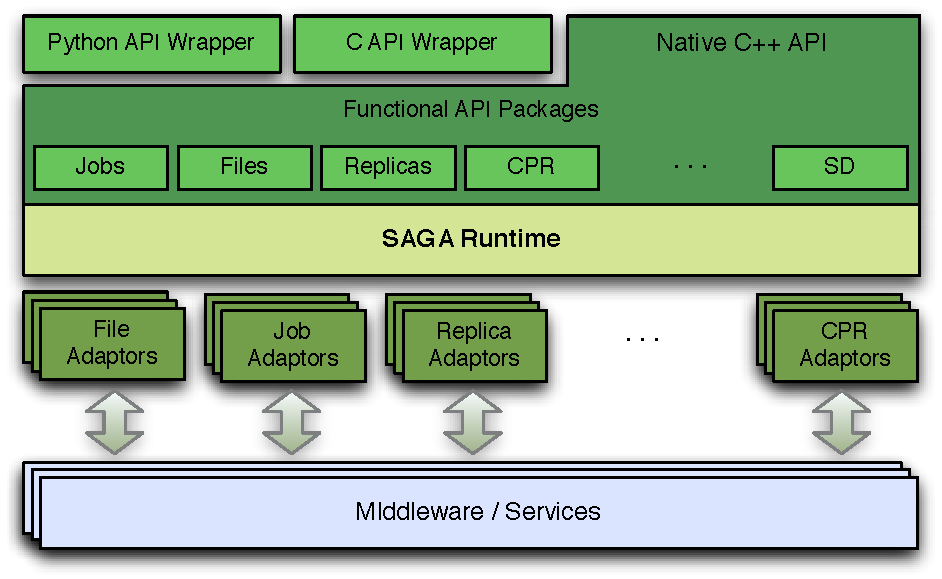
\includegraphics[scale=0.5]{saga-figure02.pdf}
\caption{In addition to the programmer's interface,
  the other important components of the landscape are the SAGA engine,
  and functional adaptors.} \vspace{-2em}
\label{saga_figure}
\end{figure}

Fig.~\ref{saga_figure} provide a view of the SAGA landscape, and the
main functional areas that SAGA provides a standardized interface
to. Based upon an analysis of more than twenty applications, the most
commonly required functionality involve job submission across
different distributed platforms, support for file access and transfer,
as well as logical file support. Less common, but equally critical,
wherever they were required, is the support for Checkpoint and
Recovery (CPR) and Service Discovery (SD).  The API is written in C++
with Python, C and Java language support. The {\it engine} is the main
library, which provides dynamic support for run-time environment
decision making through loading relevant adaptors. We will not discuss
details of SAGA here; details can be found elsewhere~\cite{saga_url}.

\jhanote{Include only if there is space: Some of the programming
  models that are common to both data-intensive application and
  Cloud-based computing, where there is an explicit cost-model for
  data-movement, is to develop general heuristics on how we handle
  common considerations such as when to move the data to the machine
  or when to process it locally.}

\subsection{Maybe  a subsection or a paragraph on the role of Adaptors}

Forward reference the section on the role of adaptors.. 


\section{Clouds: An Emerging Distributed Infrastructure}

In our opinion the primary distinguishing feature of Grids and
Clouds  is...


\subsection{Amazon EC2:}

\subsection{Eucalyptus}

\subsection{Nimbus}



\section{Patterns for Data-Intensive Computing: MapReduce and
  All-Pairs}

In this paper we will demonstrate the use of SAGA in implementing well
known programming patterns for data intensive computing.
Specifically, we have implemented MapReduce and the
All-Pairs~\cite{allpairs_short} patterns, and have used their
implementations in SAGA to to solve commonly encountered genomic
tasks.  We have also developed real scientific applications using SAGA
based implementations of these patterns: multiple sequence alignment
can be orchestrated using the SAGA-All-pairs implementation, and
genome searching can be implemented using SAGA-MapReduce.

\jhanote{Only if space permits: We will discuss other performance
  issues that arise when implementing abstractions specific for
  data-intensive computing.  A grid application's design should not
  focus on the bandwidth of the network, the dispatch latency, the
  number of machines available, and data reliability.  Even something
  as simple as process size can be a tough challenge to optimize.  If
  a job is too small, then network traffic becomes a bottleneck and
  the design is inefficient.  If a job is too large, it is difficult
  to tell when it is hanging or still computing.  Also, if another job
  with a higher priority takes a machine over, the application will be
  waiting on jobs longer.  The main point of this paper is to show how
  a flexible, extensible implementation of programming data-intensive
  abstractions using SAGA can shield the application developer from
  many of these considerations, while still providing the
  sophisticated end-user the ability to control these performance and
  cost critical/determining factors.}

{\bf MapReduce: } MapReduce~\cite{mapreduce-paper} is a programming
framework which supports applications which operate on very large data
sets on clusters of computers.  MapReduce relies on a number of
capabilities of the underlying system, most related to file
operations.  Others are related to process/data
allocation. % The Google File-System, and other
% distributed file-systems (DFS), provide the relevant capabilities,
% such as atomic file renames.  Implementations of MapReduce on these
% DFS are free to focus on implementing the data-flow pipeline, which is
% the algorithmic core of the MapReduce framework.  
One feature worth noting in MapReduce is that the ultimate dataset is
not on one machine, it is partitioned on multiple machines distributed
over a Grid. Google uses their distributed file system (Google File
System) to keep track of where each file is located.  Additionally,
they coordinate this effort with Bigtable.

{\bf SAGA-MapReduce Implementation:} We have recently implemented
MapReduce in SAGA, where the system capabilities required by MapReduce
are usually not natively supported. Our implementation interleaves the
core logic with explicit instructions on where processes are to be
scheduled.  The advantage of this approach is that our implementation
is no longer bound to run on a system providing the appropriate
semantics originally required by MapReduce, and is portable to a
broader range of generic systems as well.  The drawback is that our
implementation is relatively more complex -- it needs to add system
semantic capabilities at some level, and it is inherently slower -- as
it is difficult to reproduce system-specific optimizations to work
generically.
% it is for these capabilities very difficult or near impossible to
% obtain system level performance on application level. 
Critically however, none of these complexities are transferred to the
end-user, and they remain hidden within the framework. Also many of
these are due to the early-stages of SAGA and incomplete
implementation of features, and not a fundamental limitation of the
design or concept of the interface or programming models that it
supports.

The overall architecture of the SAGA-MapReduce implementation is shown
in Fig.~\ref{saga-mapreduce_controlflow}. This simple interface
provides the complete functionality needed by any MapReduce algorithm,
while hiding the more complex functionality, such as chunking of the
input, sorting of the intermediate results, launching and coordinating
the map and reduce workers, etc. as implemented by the framework.  The
application consists of two independent processes, a master and worker
processes. The master process is responsible for:

\begin{figure}[t]
\upp
\centering
%          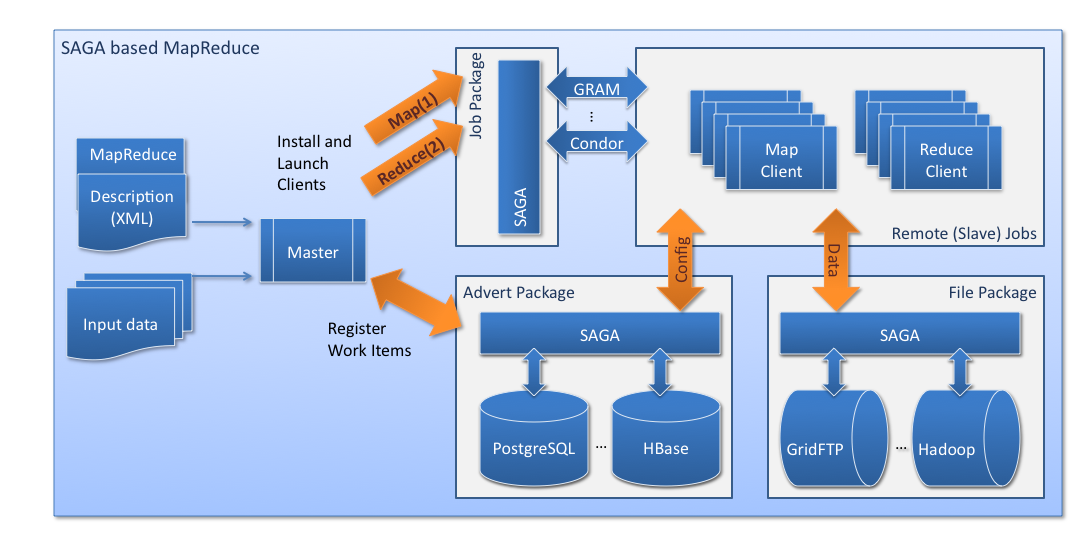
\includegraphics[width=0.4\textwidth]{saga-mapreduce_controlflow.png}
\caption{High-level control flow diagram for SAGA-MapReduce. SAGA uses
  a master-worker paradigm to implement the MapReduce pattern. The
  diagram shows that there are several different infrastructure
  options to a SAGA based
  application; % in particular for MapReduce there
  \jhanote{I think there should be something between the Map(1) and
    the Reduce(2) phases.. something that comes back to the Master,
    non?}} \vspace{-2em}
      \label{saga-mapreduce_controlflow}
\end{figure}

\begin{itemize}
\item Launching all workers for the map and reduce steps as described
  in a configuration file provided by the user 
\item Coordinating the executed workers, including the chunking of the
  data, assigning the input data to the workers of the map step,
  handling the intermediate data files produced by the map step and
  passing the names of the sorted output files to the workers of the
  reduce step, and collecting the generated outputs from the reduce
  steps and relaunching single worker instances in case of failures,
\end{itemize}

The master process is readily available to the user and needs no
modification for different Map and Reduce functions to execute.  The
worker processes get assigned work either from the map or the reduce
step. The functionality for the different steps have to be provided by
the user, which means the user has to write 2 C++ functions
implementing the required MapReduce algorithm.
Fig.\ref{src:saga-mapreduce} shows a very simple example of a
MapReduce application to count the word frequencies in the
input data set. The user provided functions |map| (line 14) and
|reduce| (line 25) are invoked by the MapReduce framework during the
map and reduce steps. The framework provides the URL of the input data
chunk file to the |map| function, which should call the function
|emitIntermediate| for each of the generated output key/value pairs
(here the word and it's count, i.e. '1', line 19). During the
reduce step, after the data has been sorted, this output data is
passed to the |reduce| function. The framework passes the key and a
list of all data items which have been associated with this key during
the map step. The reduce step calls the |emit| function
(line 34) for each of the final output elements (here: the word
and its overall count). All key/value pairs that are passed to |emit|
will be combined by the framework into a single output file.

% \begin{figure}[!ht]
%  \begin{center}
%   \begin{mycode}[label=SAGA MapReduce Word Count Algorithm]
%   // Counting words using SAGA-MapReduce
%   using namespace std;
%   using namespace boost;

%   class CountWords 
%     : public MapReduceBase<CountWords> {
%   public:
%     CountWords(int argc, char *argv[]) 
%       : MapReduceBase<CountWords>(argc, argv) 
%     {}

%     // Separate input into words
%     // Input:  url of input chunk (chk)
%     // Output: separated words and associated 
%     //         data (here: '1')
%     void map(saga::url chk) {
%       using namespace boost::iostreams;
%       stream<saga_file_device> in(chk.str());
%       string elem;
%       while(in >> elem) 
%         emitIntermediate(elem, "1");
%     } 

%     // Count words
%     // Input:  word to count (key)
%     //         list of associated data items
%     // Output: words and their count
%     void reduce(string const& key, 
%       vector<string> const& values) {
%       typedef vector<string>::iterator iter;

%       int result = 0;
%       iter end = values.end();
%       for (iter it = values.begin(); 
%            it != end; ++it) {
%         result += lexical_cast<int>(*it);
%       }
%       emit(key, lexical_cast<string>(result));
%     }
%   };
%   \end{mycode}
%   \caption{\label{src:saga-mapreduce} Counting word frequencies using
%     SAGA-MapReduce. This is the worker-side code.}
%  \end{center}
% \end{figure}

As shown in Fig.~\ref{saga-mapreduce_controlflow} both, the master and
the worker processes use the SAGA-API as an abstract interface to the
used infrastructure, making the application portable between different
architectures and systems. The worker processes are launched using the
SAGA job package, allowing to launch the jobs either locally, using
Globus/GRAM, Amazon Web Services, or on a Condor pool. The
communication between the master and the worker processes is ensured
by using the SAGA advert package, abstracting an information database
in a platform independent way (this can also be achieved through
SAGA-Bigtable adaptors).  The Master process creates partitions of
data (referred to as chunking, analogous to Google's MapReduce), so
the data-set does not have to be on one machine and can be
distributed; this is an important mechanism to avoid limitations in
network bandwidth and data distribution.  These files could then be
recognized by a distributed File-System (FS) such as Hadoop-FS
(HDFS). All file transfer operations are based on the SAGA file
package, which supports a range of different FS and transfer
protocols, such as local-FS, Globus/GridFTP, KFS, and HDFS.

{\bf All-Pairs: } As the name suggests, All-Pairs involve comparing
every element in a set to every element in another set.  Such a
pattern is pervasive and finds utility in many domains -- including
testing the validity of an algorithm, or finding an anomaly in a
configuration.  For example, the accepted method for testing the
strength of a facial recognition algorithm is to use All-Pairs
testing.  This creates a similarity matrix, and because it is known
which images are the same person, the matrix can show the accuracy of
the algorithm.

% {\bf SAGA All-Pairs Implementation: } SAGA All-pairs implementation
% is very similar to \sagamapreduce implementation.  The main
% difference is in the way jobs are run and how the data are stored.
% In \sagamapreduce the final data is stored on many machines -- if
% there is a DFS available, whereas SAGA All-pairs uses the database
% to also store information about the job.  We decided to do this
% because all data must be available to be useful. We demonstrate the
% SAGA All-Pairs abstraction using the HDFS and GridFTP to not only
% show that SAGA allows for many different configurations, but also to
% see how these different configurations behave. We have also used a
% distributed data-store -- specifically HBase (Yahoo's implementation
% of Bigtable) in lieu of the traditional Advert Service to store the
% end-results.

% {\it Multiple Sequence Alignment Using All-Pairs:} % All-Pairs is
% An important problem in Bioinformatics -- Multiple Sequence Alignment
% (MSA), can be reformulated to use All-Pairs pattern. It uses a
% comparison matrix as a reference to compare many fragment genes to
% many base genes.  Each fragment is compared to every base gene to find
% the smallest distance -- maximum overlap.  Distance is computed by
% summing up the amount of similarity between each nucleotide of the
% fragment to each one in the base.  This is done starting at every
% point possible on the base.

\section{Interfacing SAGA to Cloud-like Infrastructure: The role of
  Adaptors}

As alluded to, there is a proliferation of Clouds and Cloud-like
systems, but it is important to remember that ``what constitutes or
does not constitute a Cloud'' is not universally agreed upon.  However
there are several aspects and attributes of Cloud systems that are
generally agreed upon~\cite{buyya_hpcc}...

% Here we will by necessity
% limit our discussion to two type of distributed file-systems (HDFS and
% KFS) and two types of distributed structured-data store (Bigtable and
% HBase). We have developed SAGA adaptors for these, have used
% \sagamapreduce (and All-Pairs) seamlessly on these infrastructure.

% {\it HDFS and KFS: } HDFS is a distributed parallel fault tolerant
% application that handles the details of spreading data across multiple
% machines in a traditional hierarchical file organization.  Implemented
% in Java, HDFS is designed to run on commodity hardware while providing
% scalability and optimizations for large files.  The FS works by having
% one or two namenodes (masters) and many rack-aware datanodes (slaves).
% All data requests go through the namenode that uses block operations
% on each data node to properly assemble the data for the requesting
% application.  The goal of replication and rack-awareness is to improve
% reliability and data retrieval time based on locality.  In data
% intensive applications, these qualities are essential. KFS (also
% called CloudStore) is an open-source high-performance distributed FS
% implemented in C++, with many of the same design features as HDFS.

% There exist many other implementations of both distributed FS (such as
% Sector) and of distributed data-store (such as Cassandra and
% Hybertable); for the most part they are variants on the same theme
% technically, but with different language and performance criteria
% optimizations.  Hypertable is an open-source implementation of
% Bigtable; Cassandra is a Bigtable clone but eschews an explicit
% coordinator (Bigtable's Chubby, HBase's HMaster, Hypertable's
% Hyperspace) for a P2P/DHT approach for data distribution and location
% and for availability.  In the near future we will be providing
% adaptors for Sector\footnote{http://sector.sourceforge.net/} and
% Cassandra\footnote{http://code.google.com/p/the-cassandra-project/}.
% And although Fig.~\ref{saga_figure} explicitly maps out different
% functional areas for which SAGA adaptors exist, there can be multiple
% adaptors (for different systems) that implement that functionality;
% the SAGA run-time dynamically loads the correct adaptor, thus
% providing both an effective abstraction layer as well as an
% interesting means of providing interoperability between different
% Cloud-like infrastructure.  As testimony to the power of SAGA, the
% ability to create the relevant adaptors in a lightweight fashion and
% thus extend applications to different systems with minimal overhead is
% an important design feature and a significant requirement so as to be
% an effective programming abstraction layer.

\subsection{Clouds Adaptors: Design and Implementation}


\section{SAGA: An interface to Clouds and Grids}


The total time to completion ($T_c$) of a \sagamapreduce job, can be
decomposed into three primary components: $t_{pp}$ defined as the time
for pre-processing -- which in this case is the time to chunk into
fixed size data units, and to possibly distribute them. This is in
some ways the overhead of the process.  $t_{comp}$ is the time to
actually compute the map and reduce function on a given worker, whilst
$t_{coord}$ is the time taken to assign the payload to a worker,
update records and to possibly move workers to a destination
resource. $t_{coord}$ is indicative of the time that it takes to
assign chunks to workers and scales as the number of workers
increases. In general: 

\vspace{-1em}
\begin{eqnarray}
T_c = t_{pp} + t_{comp} + t_{coord}
\end{eqnarray}

To establish the effectiveness of SAGA as a mechanism to develop
distributed applications, and the ability of \sagamapreduce to be
provide flexibility in distributing compute units, we have designed
the following experiment set\footnote{We have also distinguished
  between SAGA All-Pairs using Advert Service versus using HBase or
  Bigtable as distributed data-store, but due to space constraints we
  will report results of the All-Pairs experiments elsewhere.}  :


In an earlier paper, we had essentially done the following:
\begin{enumerate}
\item Both \sagamapreduce workers
  (compute) and data-distribution are local. Number of workers vary
  from 1 to 10, and the data-set sizes varying from 1 to 10GB. % Here we
%   will also compare \sagamapreduce with native MapReduce (using HDFS
%   and Hadoop)
\item \sagamapreduce workers compute local (to master), but using a
  distributed FS (HDFS)
% upto 3 workers (upto a data-set size of 10GB).
\item Same as Exp. \#2, but using a different distributed FS
  (KFS); the number of workers varies from 1-10
\item \sagamapreduce using distributed compute (workers) and distributed file-system (KFS)
\item Distributed compute (workers) but using local file-systems (using GridFTP for transfer)
\end{enumerate}

In this paper, we do the following:
\begin{enumerate}
\item For Clouds the default assumption should be that the VMs are
  distributed with respect to each other. It should also be assumed
  that some data is also locally distributed (with respect to a VM).
  Number of workers vary from 1 to 10, and the data-set sizes varying
  from 1 to 10GB.  Compare performance of \sagamapreduce when
  exclusively running in a Cloud to the performance in Grids. (both
  Amazon and GumboCloud) Here we assume that the number of workers per
  VM is 1, which is treated as the base case.
\item We then vary the number of workers per VM, such that the ratio
  is 1:2; we repeat with the ratio at 1:4 -- that is the number of
  workers per VM is 4.
\item We then distribute the same number of workers across Grids and
  Clouds (assuming the base case for Clouds)
\item Distributed compute (workers) but using GridFTP for
  transfer. This corresponds to the case where workers are able to
  communicate directly with each other.
\end{enumerate}

{\bf SAGA-MapReduce on Clouds: } Thanks to the low overhead of
developing adaptors, SAGA has been deployed on three Cloud Systems --
Amazon, Nimbus~\cite{nimbus} and Eucalyptus~\cite{eucalyptus} (we have
a local installation of Eucalyptus, referred to as GumboCloud).  On
EC2, we created custom virtual machine (VM) image with preinstalled
SAGA.  For Eucalyptus and Nimbus, a boot strapping script equips a
standard VM instance with SAGA, and SAGA's prerequisites (mainly
boost).  To us, a mixed approach seemed most favourable, where the
bulk software installation is statically done via a custom VM image,
but software configuration and application deployment are done
dynamically during VM startup.

There are several aspects to Cloud Interoperability. A simple form of
interoperability -- more akin to inter-changeable -- is that any
application can use either of the three Clouds systems without any
changes to the application: the application simply needs to
instantiate a different set of security credentials for the respective
runtime environment, aka cloud.  Interestingly, SAGA provides this level of
interoperability quite trivially thanks to the adaptors.

By almost trivial extension, SAGA also provides Grid-Cloud
interoperability, as shown in Fig.~\ref{gramjob} and ~\ref{vmjob},
where exactly the same interface and functional calls lead to job
submission on Grids or on Clouds. Although syntactically identical,
the semantics of the calls and back-end management are somewhat
different.  For example, for Grids, a \texttt{job\_service} instance
represents a live job submission endpoint, whilst for Clouds it
represents a VM instance created on the fly.  It takes SAGA about 45
seconds to instantiate a VM on Eucalyptus, and about 90 seconds on
EC2. Once instantiated, it takes about 1 second to assign a job to a
VM on Eucalyptus, or EC2.  It is a configurable option to tie the VM
lifetime to the \texttt{job\_service} object lifetime, or not.

We have also deployed \sagamapreduce to work on Cloud platforms.  It
is critical to mention that the \sagamapreduce code did not undergo
any changes whatsoever. The change lies in the run-time system and
deployment architecture. For example, when running \sagamapreduce on
EC2, the master process resides on one VM, while workers reside on
different VMs.  Depending on the available adaptors, Master and Worker
can either perform local I/O on a global/distributed file system, or
remote I/O on a remote, non-shared file systems.  In our current
implementation, the VMs hosting the master and workers share the same
ssh credentials and a shared file-system (using sshfs/FUSE).
Application deployment and configuration (as discussed above) are also
performed via that sshfs.  Due to space limitations we will not
discuss the performance data of \sagamapreduce with different data-set
sizes and varying worker numbers.

\begin{figure}[!ht]
\upp
 \begin{center}
  \begin{mycode}[label=SAGA Job Launch via GRAM gatekeeper]
   { // contact a GRAM gatekeeper
    saga::job::service     js;
    saga::job::description jd;
    jd.set_attribute (``Executable'', ``/tmp/my_prog'');
    // translate job description to RSL
    // submit RSL to gatekeeper, and obtain job handle
    saga:job::job j = js.create_job (jd);
    j.run ():
    // watch handle until job is finished
    j.wait ();
   } // break contact to GRAM
  \end{mycode}
  \caption{\label{gramjob}Job launch via Gram }
 \end{center}
\upp
\end{figure}


\begin{figure}[!ht]
\upp
 \begin{center}
  \begin{mycode}[label=SAGA create a VM instance on a Cloud]
   {// create a VM instance on Eucalyptus/Nimbus/EC2
    saga::job::service     js;
    saga::job::description jd;
    jd.set_attribute (``Executable'', ``/tmp/my_prog'');
    // translate job description to ssh command
    // run the ssh command on the VM
    saga:job::job j = js.create_job (jd);
    j.run ():
    // watch command until done
    j.wait ();
   } // shut down VM instance
  \end{mycode}
  \caption{\label{vmjob} Job launch via VM}
 \end{center}
\upp
\end{figure}


{\bf SAGA-MapReduce on Clouds and Grids:} 
\begin{figure}[t]
  % 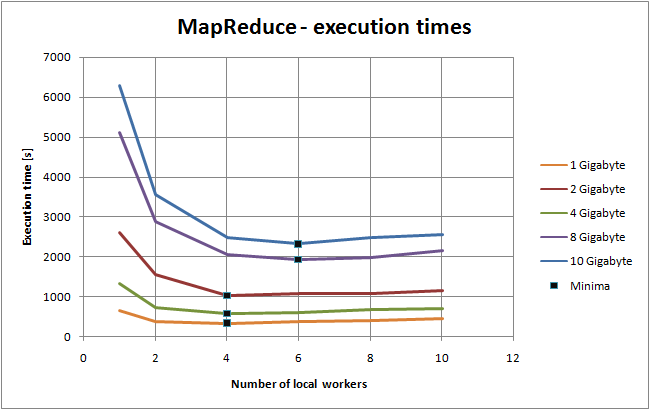
\includegraphics[width=0.4\textwidth]{MapReduce_local_executiontime.png}
  \caption{Plots showing how the \tc for different data-set sizes
    varies with the number of workers employed.  For example, with
    larger data-set sizes although $t_{pp}$ increases, as the number
    of workers increases the workload per worker decreases, thus
    leading to an overall reduction in $T_c$. The advantages of a
    greater number of workers is manifest for larger data-sets.}
\label{grids1}
\upp
\upp
\upp
\upp
\upp
\upp
\upp
\upp
\end{figure}


{\bf SAGA-MapReduce on Cloud-like infrastructure: } Accounting for the
fact that time for chunking is not included, Yahoo's MapReduce takes a
factor of 2 less time than \sagamapreduce
(Fig.~\ref{mapreduce_timing_FS}). This is not surprising, as
\sagamapreduce implementations have not been optimized, e.g.,
\sagamapreduce is not multi-threaded.
\begin{figure}[t]
\upp
      \centering
%          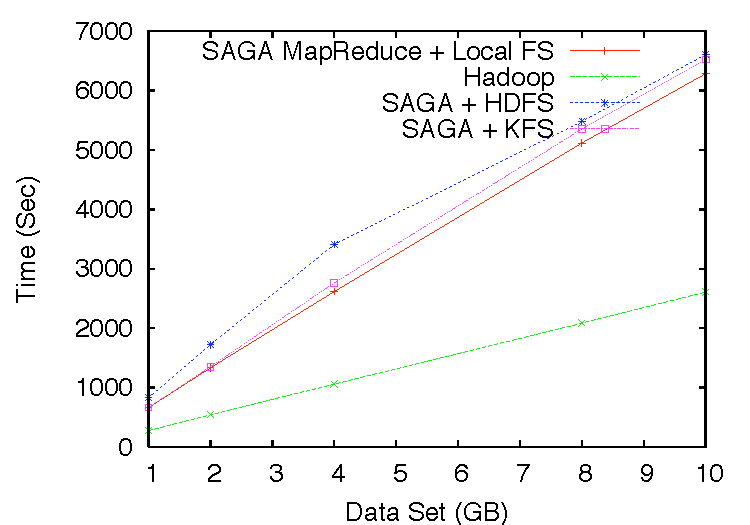
\includegraphics[width=0.40\textwidth]{mapreduce_timing_FS.pdf}
          \caption{\tc for \sagamapreduce using one worker (local to
            the master) for different configurations.  The label
            ``Hadoop'' represents Yahoo's MapReduce implementation;
            \tc for Hadoop is without chunking, which takes
            several hundred sec for larger data-sets.  The ``SAGA
            MapReduce + Local FS'' corresponds to the use of the local
            FS on Linux clusters, while the label ``SAGA + HDFS''
            corresponds to the use of HDFS on the clusters. Due to
            simplicity, of the Local FS, its performance beats
            distributed FS when used in local mode.}
          % It is interesting to note that as the data-set sizes get
          % larger, HDFS starts outperforming local FS.  We attribute
          % this to the use of caching and other advanced features in
          % HDFS which prove to be useful, even though it is not being
          % used in a distributed fashion.  scenarios considered are
          % (i) all infrastructure is local and thus SAGA's local
          % adapters are invoked, (ii) local job adaptors are used,
          % but the hadoop file-system (HDFS) is used, (iii) Yahoo's
          % mapreduce.
%      \label{saga_mapreduce_1worker.png}
          \label{mapreduce_timing_FS}
\upp
\end{figure}
Experiment 5 (Table~\ref{exp4and5}) provides insight into performance
figure when the same number of workers are available, but are either
all localized, or are split evenly between two similar but distributed
machines. It shows that to get lowest $T_c$, it is often required to
both distribute the compute and lower the workload per worker; just
lowering the workload per worker is not good enough as there is still
a point of serialization (usually local I/O).  % It shows that when
% workload per worker gets to a certain point, it is beneficial to
% distribute the workers, as the machine I/0 becomes the bottleneck.
When coupled with the advantages of a distributed FS, the ability to
both distribute compute and data provides additional performance
advantage, as shown by the values of $T_c$ for both distributed
compute and DFS cases in Table~\ref{exp4and5}.

\begin{table}
\upp
\begin{tabular}{ccccc}
  \hline
  \multicolumn{2}{c}{Configuration}  &  data size   &   work-load/worker & $T_c$  \\

  compute &  data &   (GB)  & (GB/W) & (sec) \\
  \hline
%   local   & 1 & 0.5 & 372 \\
%   \hline
%   distributed   & 1  & 0.25 & 372 \\
%   \hline \hline
  local & local-FS & 1 & 0.1 & 466 \\
  \hline
  distributed & local-FS & 1 & 0.1 & 320 \\
  \hline
  distributed & DFS & 1 & 0.1 &  273.55 \\
  \hline \hline
  local & local-FS & 2 & 0.25 & 673 \\
  \hline 
  distributed & local-FS & 2 & 0.25 & 493 \\
  \hline
  distributed & DFS & 2 & 0.25 &  466 \\
  \hline \hline
  local & local-FS &  4 & 0.5 & 1083\\
  \hline
  distributed & local-FS &  4 &  0.5&  912 \\
  \hline
  distributed & DFS & 4 & 0.5 &  848  \\
  \hline \hline
\end{tabular}
\upp
\caption{Table showing \tc for different configurations of compute  
  and data. The two compute configurations correspond to the situation
  where all workers are either
  placed locally or  workers are distributed across two different resources. The data configurations arise when using a single local FS  or a distributed FS  (KFS) with 2 data-servers. It is evident from performance figures that an optimal value arises when distributing both data and compute.}  \label{exp4and5}
\upp
\upp
\end{table}


\section{Conclusion}
We have demonstrated the power of SAGA as a programming interface and
as a mechanism for codifying computational patterns, such as MapReduce
and All-Pairs.  Patterns capture a dominant and recurring
computational mode; by providing explicit support for such patterns,
end-users and domain scientists can reformulate their scientific
problems/applications so as to use these patterns. % For example, we
% have shown how traditional applications such as MSA and Gene Search
% can be implemented using the All-Pairs and MapReduce patterns.
This
provides further motivation for abstractions at multiple-levels.
%support basic functionality but also data-intensive patterns.
We have shown the power of abstractions for data-intensive computing 
% patterns and
% abstractions
% that support such patterns, 
by demonstrating how SAGA, whilst providing the required controls and
supporting relevant programming models, can decouple the development
of applications from the deployment and details of the run-time
environment.

\section{Acknowledgments}

SJ acknowledges UK EPSRC grant number GR/D0766171/1 for supporting
SAGA and the e-Science Institute, Edinburgh for the research theme,
``Distributed Programming Abstractions''.  This work would not have
been possible without the efforts and support of other members of the
SAGA team.  In particular, \sagamapreduce was written by Chris and
Michael Miceli with assistance from Hartmut Kaiser.  We also
acknowledge internal resources of the Center for Computation \&
Technology (CCT) at LSU and computer resources provided by LONI.
\bibliographystyle{plain} \bibliography{saga_data_intensive}
\end{document}

\jhanote{We begin with the observation that the efficiency of \sagamapreduce is
pretty close to 1, actually better than 1 -- like any good (data)
parallel applications should be.  For 1GB data-set, \tc = 659s and for
10GB \tc = 6286s.  The efficiency remains at or around 1, even when
the compute is distributed over two machines: 1 worker at each site:
\tc = 672s, \tc = 1081s and \tc =2051s for 1, 2 and 4GB respectively;
this trend is valid even when the number of workers per site is more
than 1.

Fig.~\ref{grids1} plots the \tc for different number of active workers
on different data-set sizes; the plots can be understood using the
framework provided by Equation 1. For each data-set (from 1GB to 10GB)
there is an overhead associated with chunking the data into 64MB
pieces; the time required for this scales with the number of chunks
created.  Thus for a fixed chunk-size (as is the case with our
set-up), $t_{pp}$ scales with the data-set size. As the number of
workers increases, the payload per worker decreases and this
contributes to a decrease in time taken, but this is accompanied by a
concomitant increase in $t_{coord}$. However, we will establish that
the increase in $t_{coord}$ is less than the decrease in
$t_{comp}$. Thus the curved decrease in \tc can be explained by a
speedup due to lower payload as the number of workers increases whilst
at the same time the $t_{coord}$ increases; although the former is
linear, due to increasing value of the latter, the effect is a
curve. The plateau value is dominated by $t_{pp}$ -- the overhead of
chunking etc, and so increasing the number of workers beyond a point
does not lead to a further reduction in \tc.

To take a real example, we consider two data-sets, of sizes 1GB and
5GB and vary the chunk size, between 32MB to the maximum size
possible, i.e., chunk sizes of 1GB and 5GB respectively. In the
configuration where there is only one chunk, $t_{pp}$ should be
effectively zero (more likely a constant), and \tc will be dominated
by the other two components -- $t_{comp}$ and $t_{coord}$.  For 1GB
and 5GB, the ratio of \tc for this boundary case is very close to 1:5,
providing strong evidence that the $t_{comp}$ has the bulk
contribution, as we expect $t_{coord}$ to remain mostly the same, as
it scales either with the number of chunks and/or with the number of
workers -- which is the same in this case.  Even if $t_{coord}$ does
change, we do not expect it to scale by a factor of 5, while we do
expect $t_{comp}$ to do so.}

